\documentclass[12pt]{article}
\usepackage[utf8]{inputenc}
\usepackage[T1]{fontenc}
\usepackage[italian]{babel}
\usepackage{hyperref}
\usepackage{enumitem}
\usepackage{graphicx}
\usepackage{geometry}
\geometry{a4paper, margin=2.5cm}

\begin{document}

% --- PAGINA 1: FRONTESPIZIO ---
\begin{titlepage}
    \enlargethispage{3.5cm}
    \centering
    \vspace*{-2.2cm}

    % Logo dell'università
    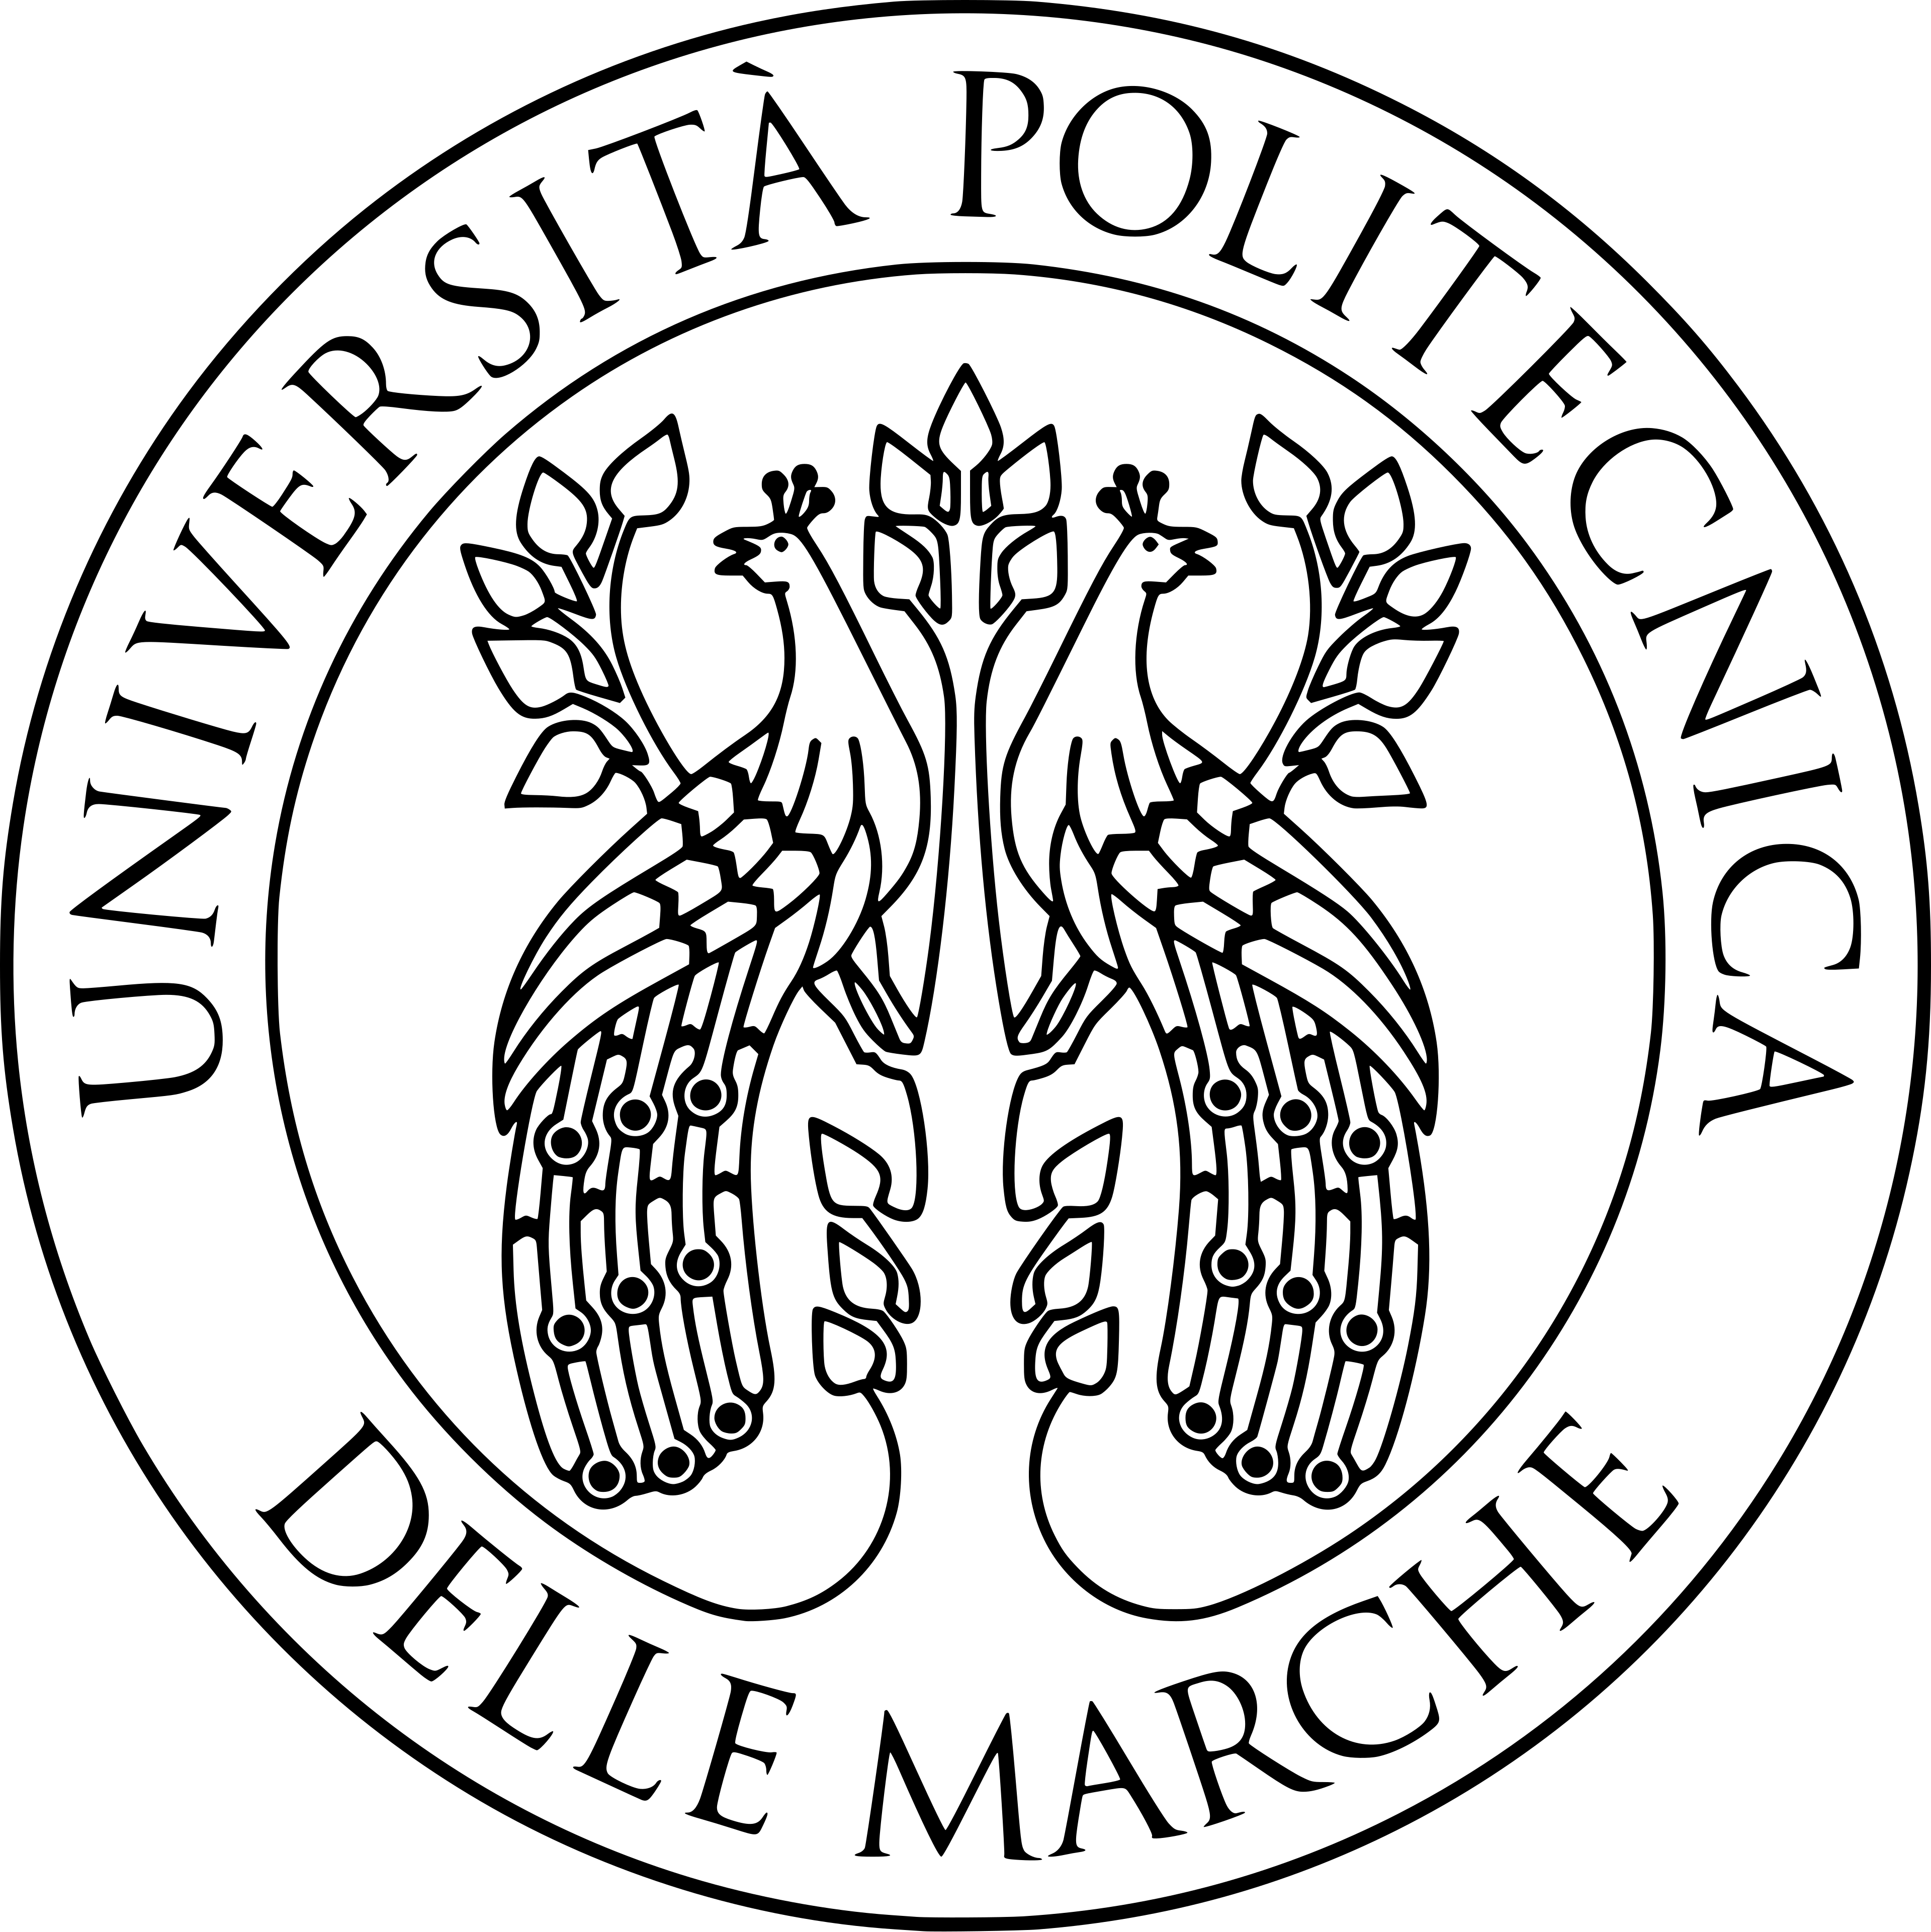
\includegraphics[width=0.28\textwidth]{logo_univpm}\par\vspace{0.2cm}

    {\Large \textbf{UNIVERSITÀ POLITECNICA DELLE MARCHE}} \par
    \vspace{0.1cm}
    {\large Corso di Laurea Triennale in Ingegneria Informatica e dell'Automazione}

    \vspace{2.5cm}

    {\large Progetto per l'esame del corso Programmazione Mobile} \par
    \vspace{0.5cm}
    {\Huge \textbf{EasyBook}} \par
    \vspace{0.2cm}
    {\large Sistema Integrato per la Gestione di Prenotazioni Professionali}

    \vfill

    \begin{flushright}
        \large
        \textbf{Autori:} \\
        Ilario Polidori \\
        Tomas Mosciatti \\
        Gianlorenzo Lucioni
    \end{flushright}

    \vspace{0.5cm}

    {\large Anno Accademico 2024/2025}

\end{titlepage}

% --- PAGINA 2: INDICE ---
\newpage
\tableofcontents
\newpage

% --- PAGINA 3 E SUCCESSIVE: CONTENUTO ---

\section{Descrizione in linguaggio naturale}

\subsection{a. Descrizione del sistema, del funzionamento e dei requisiti in linguaggio naturale}
L'applicazione \textbf{EasyBook} è un sistema gestionale mobile progettato per facilitare l'incontro tra professionisti e clienti. La piattaforma permette di digitalizzare l'intero processo di prenotazione, dalla configurazione dell'agenda aziendale fino alla recensione finale del servizio.

\textbf{Funzionamento per Ruoli:}
\begin{itemize}[noitemsep]
    \item \textbf{Manager:} Rappresenta il titolare dell'attività. Ha il compito di configurare il profilo aziendale (Business Page), caricare immagini nella galleria e descrivere i servizi. Gestisce il team invitando i collaboratori (Provider) tramite un sistema di email sicure. Dispone di una dashboard analitica per monitorare il fatturato totale e mensile, oltre alle performance dei singoli dipendenti.
    \item \textbf{Provider:} È il professionista che eroga il servizio. Definisce la propria disponibilità settimanale (giorni lavorativi e fasce orarie) e gestisce il catalogo dei servizi a lui assegnati. Riceve prenotazioni in tempo reale e ne aggiorna lo stato (es. da "Pending" a "Completed").
    \item \textbf{Client:} L'utente finale. Attraverso una ricerca per categorie o parole chiave, scopre le aziende, ne visualizza il team e la galleria immagini. Prenota servizi scegliendo data e ora da un calendario dinamico che esclude automaticamente gli slot già occupati o al di fuori dell'orario lavorativo.
\end{itemize}

\textbf{Caratteristiche Principali:}
\begin{itemize}[noitemsep]
    \item \textbf{Sicurezza:} Autenticazione Firebase con obbligo di verifica email per prevenire accessi fraudolenti.
    \item \textbf{Real-time:} Sincronizzazione immediata dei dati tra Client, Provider e Manager grazie a Firebase Firestore.
    \item \textbf{Personalizzazione:} Ogni azienda ha una pagina dedicata con galleria multimediale e catalogo completo.
\end{itemize}

\subsection{b. Glossario dei termini}
\begin{description}[noitemsep]
    \item[Client] Utente che richiede servizi e gestisce le proprie prenotazioni.
    \item[Provider] Professionista che eroga i servizi e gestisce la propria disponibilità oraria.
    \item[Manager] Supervisore aziendale con privilegi di analisi dati e gestione del personale.
    \item[Business] Entità che aggrega i servizi e i professionisti sotto un unico brand aziendale.
    \item[Booking] Record che formalizza una prenotazione, con stati: \textit{Pending, Confirmed, Completed, Canceled, Rejected}.
    \item[Slot] Intervallo temporale minimo selezionabile (es. 30 minuti) all'interno dell'orario lavorativo.
    \item[Turnover (Fatturato)] Somma economica calcolata dinamicamente sui servizi in stato "Completed".
    \item[Firestore] Database NoSQL cloud utilizzato per la memorizzazione e sincronizzazione dei dati, dei servizi e degli utenti.
\end{description}

\newpage
\section{Analisi dei requisiti}
\subsection{a. Requisiti funzionali}
I requisiti funzionali descrivono le capacità del sistema divise per attore:
\begin{itemize}
    \item \textbf{Sistema Generale:} Registrazione multi-ruolo, login, logout, recupero password e verifica email.
    \item \textbf{Manager:} Setup del Business (Nome, Categoria, Indirizzo), gestione galleria immagini, invito Provider, dashboard statistiche (fatturato, performance team, servizi popolari).
    \item \textbf{Provider:} Gestione catalogo servizi (aggiunta/modifica/eliminazione), impostazione orario settimanale, gestione agenda prenotazioni, monitoraggio fatturato personale.
    \item \textbf{Client:} Ricerca aziende/servizi, filtri per macro-categorie, visualizzazione dettagli business (team, gallery, prezzi), prenotazione tramite calendario dinamico, storico prenotazioni, inserimento recensioni.
\end{itemize}

\subsection{b. Requisiti non funzionali}
\begin{itemize}
    \item \textbf{Disponibilità:} Il sistema deve essere accessibile 24/7 grazie all'infrastruttura Cloud di Firebase.
    \item \textbf{Affidabilità:} Le transazioni di prenotazione devono garantire la coerenza dei dati (evitare il \textit{double-booking}).
    \item \textbf{Usabilità:} L'interfaccia deve essere intuitiva e seguire i pattern Material 3 di Google.
    \item \textbf{Prestazioni:} Il caricamento delle immagini aziendali deve essere fluido (uso di caching asincrono).
    \item \textbf{Portabilità:} Supporto a dispositivi con Android API 24 o superiori.
\end{itemize}

\subsection{c. Diagrammi dei casi d’uso}
\textit{[In questa sezione andranno inseriti i grafici che mostrano le interazioni degli attori con le funzionalità descritte sopra, come la gestione delle prenotazioni e l'analisi dei dati per il Manager.]}

\subsection{d. Matrice di mapping}
\textit{[Tabella che collega i Requisiti Funzionali ai corrispondenti casi d'uso e componenti software del sistema.]}

\newpage
\section{Descrizione tecnica}

\subsection{a. Tecnologie utilizzate}
Lo sviluppo di EasyBook si basa su tecnologie moderne dedicate alla realizzazione di applicazioni Android native:
\begin{itemize}
    \item \textbf{Kotlin:} linguaggio di programmazione principale utilizzato per implementare la logica dell'applicazione, i modelli dei dati e la comunicazione con i servizi Firebase.
    \item \textbf{Jetpack Compose:} toolkit dichiarativo impiegato per costruire l'interfaccia grafica. Le schermate vengono aggiornate automaticamente quando cambia lo stato osservato dalla UI.
    \item \textbf{Firebase Authentication:} servizio utilizzato per la registrazione, il login, il recupero della password e la verifica dell'indirizzo email degli utenti.
    \item \textbf{Firebase Firestore:} database NoSQL cloud nel quale vengono memorizzati utenti, Business, servizi, disponibilità, prenotazioni e recensioni. I listener real-time consentono di ricevere automaticamente gli aggiornamenti dei dati osservati.
    \item \textbf{Firebase Storage:} servizio dedicato alla memorizzazione delle immagini dei profili aziendali e delle relative gallerie multimediali.
    \item \textbf{Kotlin Coroutines:} strumento impiegato per eseguire in modo asincrono le operazioni di rete e di accesso al database senza bloccare il thread principale.
    \item \textbf{StateFlow:} flusso di stato osservabile utilizzato dai ViewModel per comunicare alla UI dati e variazioni dello stato applicativo.
    \item \textbf{Material 3:} sistema di design adottato per garantire coerenza grafica, accessibilità e uniformità dei componenti dell'interfaccia.
\end{itemize}

\subsection{b. Architettura del sistema}
L'applicazione adotta il pattern architetturale \textbf{Model--View--ViewModel (MVVM)}, che separa la rappresentazione grafica, la logica applicativa e i dati. Questa suddivisione rende il codice più leggibile, manutenibile e facilmente verificabile.

L'organizzazione logica dei package rispecchia le responsabilità dei diversi componenti:
\begin{itemize}
    \item \textbf{Model:} contiene le classi Kotlin che rappresentano le entità del dominio, come utenti, Business, servizi, prenotazioni, recensioni e disponibilità.
    \item \textbf{ViewModel:} contiene \textit{AuthViewModel}, \textit{ClientViewModel}, \textit{ProviderViewModel} e \textit{ManagerViewModel}. Questi componenti gestiscono la logica dei diversi ruoli, elaborano i dati e mantengono lo stato delle schermate.
    \item \textbf{View/UI:} comprende le schermate realizzate con Jetpack Compose, i componenti grafici riutilizzabili e la navigazione mediante \textit{NavHost}.
    \item \textbf{Data:} gestisce l'accesso a Firebase Authentication, Firestore e Storage, isolando le operazioni di persistenza dalla UI.
\end{itemize}

Il flusso dei dati parte dalla View, che inoltra al ViewModel le azioni compiute dall'utente. Il ViewModel applica la logica necessaria e richiede o modifica i dati su Firebase. I risultati vengono pubblicati tramite uno stato osservabile, come \textit{StateFlow}; Jetpack Compose osserva tale stato e ricompone automaticamente le parti dell'interfaccia interessate dalla modifica.

\subsection{c. Sintesi tecnica del funzionamento del sistema}
Il progetto è costruito su tre pilastri:

\begin{enumerate}
    \item \textbf{Reattività real-time (Firebase Firestore):} l'app non richiede aggiornamenti manuali. Quando un Client effettua una prenotazione, il Provider vede comparire la relativa notifica nella propria lista istantaneamente. Quando il Provider completa un servizio, le statistiche del Manager si aggiornano in tempo reale.

    \item \textbf{Architettura MVVM:}
    \begin{itemize}
        \item \textbf{Model:} semplici classi Kotlin che rappresentano i dati memorizzati nel database.
        \item \textbf{ViewModel:} costituisce il ``cuore'' logico dell'applicazione. Filtra i dati per il Client, calcola il fatturato per il Manager e genera gli orari disponibili.
        \item \textbf{View (Jetpack Compose):} interfaccia utente dichiarativa che osserva lo stato del ViewModel. Quando i dati cambiano, la UI si ridisegna automaticamente.
    \end{itemize}

    \item \textbf{Logica degli slot (algoritmo di prenotazione):} per evitare sovrapposizioni, il sistema:
    \begin{enumerate}[label=\roman*.]
        \item recupera gli orari di lavoro del professionista per il giorno della settimana selezionato;
        \item scarica tutte le prenotazioni già esistenti, escluse quelle cancellate o rifiutate;
        \item suddivide la giornata in intervalli di 30 minuti;
        \item sottrae gli intervalli già occupati e mostra al Client soltanto quelli liberi.
    \end{enumerate}
\end{enumerate}

\newpage
\section{Diagrammi di analisi}
\subsection{a. Diagramma delle classi di analisi}
Il diagramma mostrerà le relazioni tra le entità principali: \textit{User}, \textit{Business}, \textit{Service}, \textit{Booking}, \textit{Review} e \textit{Availability}.

\subsection{b. Diagrammi di sequenza}
I diagrammi descriveranno i flussi critici:
\begin{enumerate}
    \item Processo di prenotazione di un servizio da parte del cliente.
    \item Accettazione/Completamento di una prenotazione da parte del professionista.
    \item Generazione dinamica delle statistiche di fatturato nella dashboard manager.
    \item Flusso di invito di un Provider in un Business da parte del Manager.
\end{enumerate}

\subsection{c. Diagrammi di attività}
Rappresentazione logica dei processi decisionali, come la logica di generazione degli slot orari liberi.

\newpage
\section{Diagrammi di progettazione}
\subsection{a. Diagramma delle classi di progettazione}
Dettaglio delle classi Kotlin, dei ViewModel (\textit{AuthViewModel, ClientViewModel, ProviderViewModel, ManagerViewModel}) e della loro interazione con i repository Firebase.

\subsection{b. Diagramma dei componenti}
Separazione tra il modulo UI (Compose), il modulo Business Logic (ViewModels) e il modulo Data (Firebase).

\subsection{c. Diagrammi delle macchine a stati}
Descrizione del ciclo di vita della classe \textit{Booking} (stati transazionali) e dello stato di autenticazione dell'utente.

\newpage
\section{Implementazione}
\subsection{a. Diagramma di deployment}
Descrizione dell'interazione tra lo smartphone dell'utente e i server Google Cloud/Firebase.

\subsection{b. Mockup}
L'app utilizza una navigazione basata su \textit{Scaffolds} e \textit{NavHost}. La Home del cliente presenta una ricerca globale, mentre la dashboard del manager si focalizza su grafici testuali e performance del team.

\subsection{c. Gestione asincrona delle prenotazioni}
Sì, la gestione delle prenotazioni nel codice attuale è completamente asincrona, il che significa che l'app non si blocca mai durante il caricamento dei dati o il salvataggio.

Tuttavia, c'è una distinzione importante tra asincrono e reattivo (real-time) per quanto riguarda gli slot:

\begin{enumerate}
    \item \textbf{Come funziona ora (asincrono ma non reattivo per gli slot)}

    Nel file \textit{ClientViewModel.kt}, la funzione \textit{generateSlots} usa il metodo \textit{get()}:
    \begin{itemize}
        \item Quando l'utente seleziona una data, viene fatta una richiesta asincrona a Firestore per scaricare le prenotazioni esistenti.
        \item Una volta ricevuta la risposta, vengono calcolati gli slot liberi.
        \item \textbf{Il limite:} se un altro Client prenota lo stesso slot mentre l'utente ha il dialog aperto, lo slot non sparirà ``in diretta''. L'utente continuerà a visualizzarlo come disponibile finché non cambierà data o riaprirà il dialog.
    \end{itemize}

    \item \textbf{Cosa succede in caso di conflitto?}

    Attualmente, se due Client premono ``Conferma'' esattamente nello stesso momento per il medesimo orario:
    \begin{enumerate}
        \item vengono create due prenotazioni con stato \textit{Pending};
        \item il professionista (Provider) le vedrà entrambe nella propria dashboard e dovrà decidere quale accettare e quale rifiutare, gestendo manualmente il conflitto.
    \end{enumerate}
\end{enumerate}

\subsection{d. Descrizione unit tests}
\textbf{Scelte Implementative e Testing:}
\begin{itemize}
    \item \textbf{Pattern MVVM:} Scelto per separare nettamente la UI dalla logica di accesso ai dati, facilitando la manutenzione.
    \item \textbf{Gestione Asincrona:} Uso massiccio di Kotlin Coroutines per gestire le chiamate di rete senza bloccare il thread principale della UI.
    \item \textbf{Reattività delle UI:} Implementazione di \textit{StateFlow} e \textit{MutableState} per garantire che ogni modifica su Firestore si rifletta immediatamente sullo schermo dell'utente.
    \item \textbf{Algoritmo di Booking:} Logica personalizzata che incrocia la disponibilità del provider con il database delle prenotazioni correnti per filtrare gli orari in tempo reale.
\end{itemize}

\end{document}
